\section{Sistemas de Navegação por Satélites}
\label{sec:GNSS}
Nesta seção é apresentado o referencial teórico sobre Sistemas de Navegação por Satélites, seus princípios básicos, funcionamento e como podem ser aplicados no desenvolvimento da técnica adaptativa objetivada neste trabalho.

\subsection{Contexto e Definições}

A última década foi marcada pela popularização e evolução dos dispositivos móveis, principalmente os \emph{smartphones}. Esses dispositivos contam com diversas funcionalidades de software e hardware úteis para o dia a dia dos usuários, incluindo, em sua gigantesca maioria, serviços de geolocalização, que, por sua vez, dão ao usuário informações sobre a sua localização geográfica corrente.

Para o ser humano moderno, a possibilidade de saber qual a sua posição atual no mundo traz inúmeras vantagens que vão muito além de saber se está próximo de um estabelecimento que o mesmo está procurando para realizar as compras do mês. O acesso a essa informação traz a humanidade um leque de possibilidades, que são ainda mais ampliadas com o uso de uma rede de computadores. Como exemplo, podemos ter acesso à informações sobre o clima local, saber sobre os estabelecimentos próximos, calcular rotas precisas a partir da posição do usuário, associar o local a fotos e vídeos, e muito mais. Além disso, sistemas de georreferenciamento fazem o uso de imagens de satélites para determinar os limites de bairros e casas visando gerar informações de limites e posicionamento.

Existem, atualmente, dois principais Sistemas de Navegação por Satélites (do inglês "Global Navigation Satellite Systems" ou GNSS) funcionais responsáveis por permitir a descoberta de informações sobre o posicionamento de objetos no globo: O NAVSTAR-GPS (do inglês "Navigation Satellite with Time And Ranging Global Positioning System"), comumente conhecido apenas como GPS, e o GLONASS (sigla de origem russa para "Sistema de Navegação Global por Satélite"). 

%Ambos os sistemas necessitam do uso de receptores específicos, tornando obrigatório a existência de um hardware especial para cada um. \cite{vaz2013comparaccao}

\subsection{Referenciando a Posição de um Objeto no Globo}

Qualquer ponto na Terra pode ser referenciado por meio de um Sistema de Coordenadas Geográficas. De todos os modelos existentes o mais comum e prático é o baseado em linhas imaginárias conhecidas como \emph{meridianos} e \emph{paralelos}. Os meridianos cortam o globo do polo geográfico norte ao polo geográfico sul, já os paralelos são linhas ortogonais\footnote{Linhas que formam um ângulo de 90º ao se cruzarem.} aos meridianos. De todos os paralelos e meridianos que podem ser traçados na terra, destacam-se o Meridiano de Greenwich, que divide a terra em um lado ocidental e outro oriental, e o Paralelo da Linha do Equador, que divide a terra em polo sul e polo norte. \cite{fitz2008geoprocessamento}

\begin{figure}[htp!]
\centering
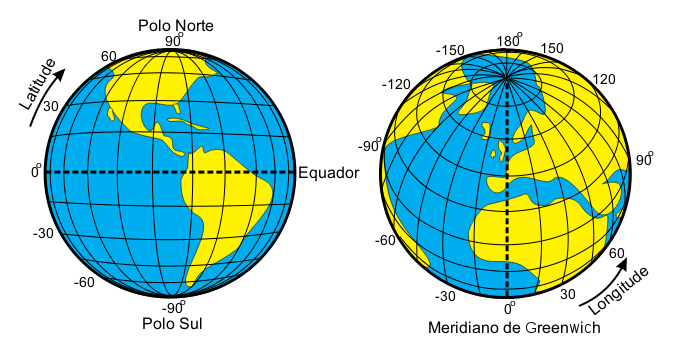
\includegraphics[width=0.80\textwidth]{figuras/cap_2/secao_3/latitude_longitude.png}
\caption{Latitude e Longitude}
\label{latitudeLingitude}
\end{figure}

A distância de qualquer ponto até a Linha do Equador é chamada de latitude e é medida em graus e varia de 0 a 90 graus, tanto para o norte (N) quanto para o sul (S). Para determinar a latitude de um ponto no globo, é preciso calcular o ângulo formado entre a linha do equador e uma reta que passa pelo ponto desejado e pelo centro da terra. Caso o ponto esteja em cima da linha do equador, não teremos a formação de um ângulo e, portanto, ele está na latitude 0º. \cite{fitz2008geoprocessamento}

Infelizmente, apenas com a latitude, não é possível determinar a posição exata de um ponto no globo. Para resolver isso é utilizada uma outra medida, a longitude. Esta medida, por sua vez, representa a distância do ponto desejado até o Meridiano de Greenwich e é calculada de forma similar a realizada para latitude, mas varia de 0 a 180 graus para leste (E) e para oeste (W). Um ponto que se localiza em cima do Meridiano de Greenwich está na longitude de 0º. \cite{fitz2008geoprocessamento}

A Figura \ref{washingtonDC} apresenta a latitude e a longitude aproximada de Washington D.C., a capital dos Estados Unidos da América.

\begin{figure}[htp!]
\centering
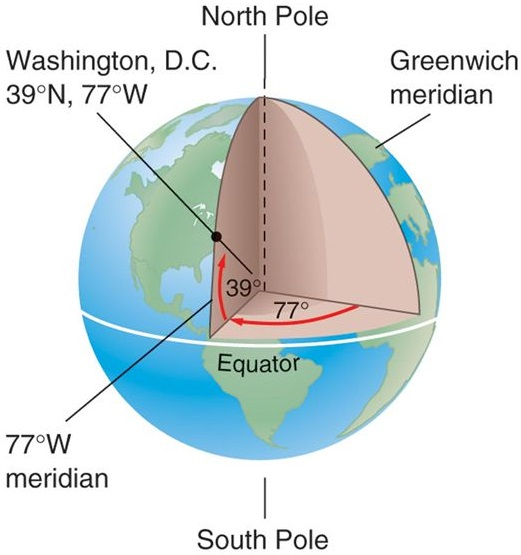
\includegraphics[width=0.60\textwidth]{figuras/cap_2/secao_3/washingtonDC.jpg}
\caption{Latitude e Longitude de Washington D.C.}
\label{washingtonDC}
\end{figure}

A distância em quilômetros de um grau a outro, que na latitude equivale a 111,12km e na longitude varia de 0 a 111,12km, torna necessário o uso de valores com várias casas decimais para representar com exatidão a posição de um objeto no globo. Para efeitos de simplificação, existe um modelo onde cada grau é dividido em duas componentes, uma de minutos (') e outra de segundos ("). Cada grau possui 60 minutos e cada minuto possui 60 segundos \cite{fitz2008geoprocessamento}. 

A divisão da latitude e da longitude em componentes torna possível simplificar a fala de uma coordenada geográfica. Como exemplo, a posição geográfica da \emph{Universidade Vila Velha} se dá na latitude 20.354043ºS e na longitude 40.299163ºW, que, quando convertido para o modelo utilizando minutos e segundos, se torna \newline 20º21'14,6"S e 40º17'57"W, respectivamente. A pronúncia do sistema em minutos e segundos é mais fácil de ser entendida e associada, pois discretiza os valores decimais muito longos que seriam necessários para referenciar um ponto no globo.

\subsection{O NAVSTAR-GPS}

O NAVSTAR-GPS, ou apenas GPS, como já foi introduzido, é uma tecnologia utilizada para determinar a posição geográfica de dispositivos no globo terrestre, fazendo uso de satélites artificiais, que funcionam como pontos de referência no espaço de posição muito bem conhecida. Além disso, foi desenvolvido pelo Departamento de Defesa dos Estados Unidos, o DOS (do inglês "Department of Defense"), está operacional desde 1994 e, devido ao tempo de operação, é mais popular em relação ao GLONASS.

A concepção do GPS permite que qualquer usuário situado na superfície terrestre, ou próximo dela, tenha a sua disposição, pelo menos, quatro satélites artificiais para serem rastreados, permitindo o conhecimento em tempo real da sua posição e uso sob condições climáticas extremas \cite{miguens1996navegaccao}. O GPS é um sistema passivo, pois não necessita que o usuário envie informações para os satélites, ficando estes responsáveis pelo envio dos sinais necessários.

Para calcular a posição de um usuário com precisão é utilizado um sistema de triangulação que faz uso da posição de três satélites e as suas respectivas distâncias até um receptor em terra. A distância do receptor até o satélite pode ser obtida por meio da medição do intervalo de tempo decorrido entre a transmissão dos sinais pelos satélites e a recepção pelo dispositivo receptor, sendo ela utilizada como raio de uma esfera cujo centro é a posição do satélite. A posição do usuário é o ponto em comum de interseção das três esferas, como ilustrado na Figura \ref{triangulacao_gps}.

\begin{figure}[htp!]
\centering
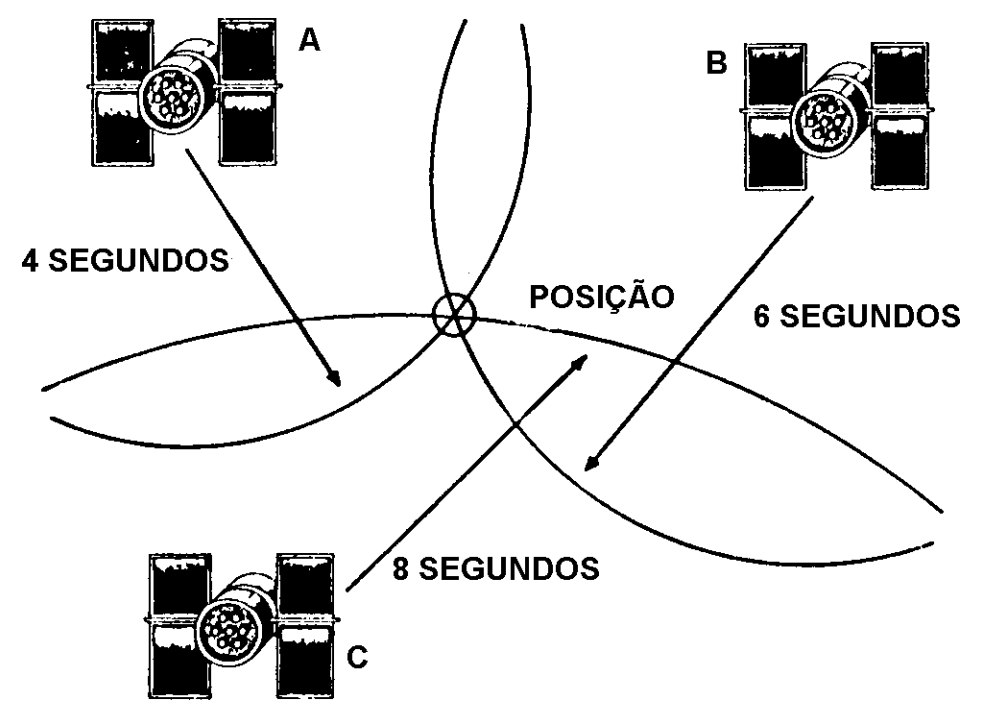
\includegraphics[width=0.60\textwidth]{figuras/cap_2/secao_3/triangulacao_gps.png}
\caption{Sistema de triangulação utilizado pelo NAVSTAR-GPS \cite{miguens1996navegaccao}.}
\label{triangulacao_gps}
\end{figure}

O cálculo do tempo decorrido entre a emissão do sinal e a recepção no dispositivo utilizado não é tão simples, pois exige a perfeita sincronização do relógio de todos os elementos envolvidos. Em situações práticas isso é muito improvável de acontecer e faz necessário o uso de mais um satélite para o processo, daí vê-se a importância da disponibilidade de, pelo menos, quatro satélites.

Não é objetivo deste trabalho realizar explanações muito específicas sobre o funcionamento do GPS. Detalhes de hardware, software e conceitos mais específicos podem ser encontrados em \cite{longley2009sistemas}.

\subsection{O GLONASS}

O GLONASS é uma tecnologia georreferenciamento de origem russa e, assim como o GPS, foi desenvolvido inicialmente para uso militar. Esse sistema só pôde ser considerado operacional em nível mundial no final 2011 e, a partir daí, começou lentamente a ser acoplado aos smartphones \cite{vaz2013comparaccao}, principalmente após o governo russo ter criado barreiras de importação para dispositivos que suportem apenas a tecnologia norte americana \cite{impostoRussia}.

O funcionamento da tecnologia russa é semelhante ao do GPS visto na Figura \ref{triangulacao_gps} e tem se tornado cada vez mais popular no mercado de dispositivos móveis e possui uma precisão muito próxima ao GPS \cite{vaz2013comparaccao}.

Até o ano de 2011, GPS e GLONASS eram totalmente incompatíveis entre-si, pois utilizavam técnicas de modulação e frequências diferentes. Entretanto, foi nesse ano que o GLONASS-K foi lançado e, por sua vez, possibilitou que dispositivos operem com as duas tecnologias utilizando um único receptor, visto que ele trabalha com frequências e modulações semelhante aos da tecnologia americana\newline \cite{kovar2011interoperable}.

\subsection{Contribuição para as Redes Tolerantes a Atrasos}

A descoberta da posição geográfica de dispositivos contribui de forma significativa em diversas áreas de pesquisa, entre elas as Redes Tolerantes a Atrasos. Conhecer a posição de cada um dos dispositivos que compõem uma DTN permite o levantamento de estatísticas de contatos ocorridos entre dispositivos em regiões preestabelecidas, abrindo mão para o gerenciamento inteligente de parâmetros que influenciam no consumo de energia dos dispositivos envolvidos.

A concentração pode ser calculada por meio da relação entre a quantidade total de contatos registrados e a quantidade de contatos ocorridos na região onde um nó se encontra. Quanto maior a concentração, maiores as chances de um dispositivo encontrar outro ao realizar uma busca e, portanto, é mais inteligente aumentar o consumo visando usufruir das oportunidades previstas. Quanto menor a concentração, menores as chances de encontrar outro dispositivo e, consequentemente, é mais inteligente economizar energia para momentos oportunos.

É importante ressaltar que o conceito de regiões apresentado na Seção \ref{sec:DTN} é diferente do que é utilizado para regiões geográficas. O primeiro refere-se a características relacionadas a protocolos, por exemplo, e aqui refere-se áreas geográficas.

\subsection{Consumo de Energia em Dispositivos Móveis}
\label{subsec:consumo_gps}
Visando o aumento da quantidade de mensagens entregues, é inerente no âmbito das DTNs tornar inteligente o consumo energético dos dispositivos. Isso implica numa análise do uso das baterias pelos dispositivos de GNSS quando considerada a contribuição proposta na Subseção anterior.

Em \cite{carroll2010analysis} foi realizado um estudo do consumo energético de diversos componentes existentes em smartphones, tais como CPU, memória RAM, memórias de armazenamento, além, é claro, de dispositivos de GPS, utilizando para isso técnicas e equipamentos de medição adequados.

Relativo ao consumo de dispositivos GPS, Carroll indica que, quando habilitados, eles consomem 143,1mW utilizando uma antena interna e 166,1mW quando utiliza-se uma antena externa. Ainda é explicitado no trabalho de Carroll que, quando desabilitados, os dispositivos GPS não realizam qualquer consumo de energia.

Outro resultado relevante apontado por Carroll é o de que não existem diferenças de consumo quando a quantidade de satélites visíveis é analisada. Sendo assim, é possível concluir que seus resultados podem ser utilizados em simulações sem a necessidade de simular a movimentação de satélites para aumentar o grau de realismo.

É visto que o estudo de Carroll é de importante valia na simulação da técnica desenvolvida neste trabalho, visto que ela baseia-se no uso de dispositivos de Georreferenciamento. Além disso, o trabalho referenciado permite aumentar o grau de realismo das simulações realizadas no que diz respeito ao consumo de energia. 

Para efeitos de simplificação, as simulações realizadas no capítulo \ref{cap:testes} consideram a média dos consumos apontados por Carrol, ou seja, 154,6mW.